\documentclass{beamer}

\usepackage[utf8]{inputenc}
\usepackage[T1]{fontenc}
\usepackage{graphicx}
\usepackage{listings}
\usepackage{xcolor}

\useinnertheme{uconn}
\useoutertheme[]{uconn}
%\useoutertheme[footline=authorinstitute,subsection=true]{miniframes}
%\useoutertheme{sidebar}
\usecolortheme{default}
\usefonttheme{default}

\title[IntroToTensorflow]{Introduction to Tensorflow for NFL Sports Analytics}
\author[Pranav]{Pranav Tavildar}
\institute[UConn]{UConn Sports Analytics Symposium 2022}
\date{\today}

\setlength{\parskip}{.5em}

\lstdefinestyle{Python}{
    language        = Python,
    basicstyle      = \tiny,
    keywordstyle    = \color{blue},
    keywordstyle    = [2] \color{teal}, % just to check that it works
    stringstyle     = \color{green},
    commentstyle    = \color{red}\ttfamily
}


\begin{document}

\lstset{
    frame       = single,
    numbers     = left,
    showspaces  = false,
    showstringspaces    = false,
}

\begin{frame}
\titlepage
\end{frame}


\begin{frame}{Table of contents}
\tableofcontents
\end{frame}

\section{Introduction to Tensorflow}

\begin{frame}[fragile]{What is Tensorflow?}

  \begin{columns}[T]
    \begin{column}{.5\textwidth}
     \begin{block}{Open Source Deep Learning Library that makes creating Models more:}
     \begin{itemize}
     % Your text here
     \item Easy
     \item Flexible
     \item Fast
     \item Reproducable
    \end{itemize}
    \end{block}
    \end{column}
    \begin{column}{.5\textwidth}
    \begin{block}{}
% Your image included here
    {
\includegraphics[width=4cm]{images/tflogo.png}}
    \end{block}
    \end{column}
  \end{columns}

\end{frame}


\begin{frame}[fragile]{The History of Tensorflow}

  \begin{columns}[T]
    \begin{column}{.5\textwidth}
     \begin{block}{Evolution of Tensorflow}
     \begin{itemize}
     % Your text here
     \item Product of Google Brain Team
     \item Evolution from Distbelief (2011)
     \item Possible because of Tensor Processing Unit
    \end{itemize}
    \end{block}
    \end{column}
    \begin{column}{.5\textwidth}
    \begin{block}{}
% Your image included here
    {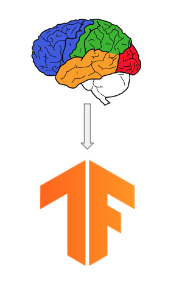
\includegraphics[width=3cm]{images/evolution.png}}
    \end{block}
    \end{column}
  \end{columns}

\end{frame}

%%%%%%%%%%%%%%%%%%
\begin{frame}[fragile]{Tensorflow vs Alternatives}
\begin{columns}[T]
 \begin{column}{.33\textwidth}
     \begin{block}{Tensorflow}
     \begin{itemize}
     \item Preferred by Companies
     \item Easily Deployable and Versatile
    \end{itemize}
     \end{block}
   \end{column}
   
    \begin{column}{.33\textwidth}
     \begin{block}{Pytorch}
     \begin{itemize}
     \item Preferred by Research Labs
     \item Easily Debuggable
    \end{itemize}
    {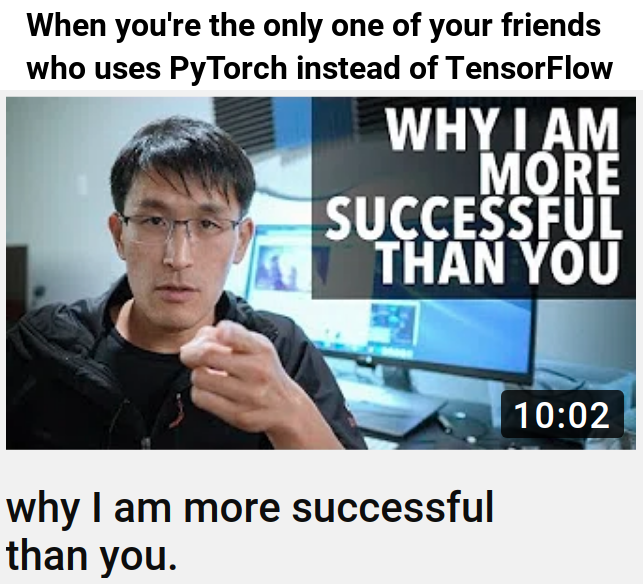
\includegraphics[width=3cm]{images/altmeme.png}}
     \end{block}
   \end{column}
   
   \begin{column}{.33\textwidth}
     \begin{block}{Caffe}
     \begin{itemize}
     \item Used by Researchers and Startups
     \item Useful for Small but Specific and fast use cases
    \end{itemize}
     \end{block}
   \end{column}

\end{columns}
\end{frame}

\begin{frame}[fragile]{What is a Tensor?}
\begin{itemize}
	\item Tensor is data with dimension.
	\item 0-d tensor: scalar
	\begin{equation*}
	c = 5
	\end{equation*} 
	\item 1-d tensor: vector
	\begin{equation*}
	{\rm{c}} = \left( {\begin{array}{*{20}{c}}
1\\
 \vdots \\
5
\end{array}} \right)
	\end{equation*} 
	\item 2-d tensor: matrix
	\begin{equation*}
	{\rm{c}} = \left( {\begin{array}{*{20}{c}}
1& \cdots &5\\
 \vdots & \ddots & \vdots \\
5& \cdots &5
\end{array}} \right)
	\end{equation*}
\end{itemize}
\end{frame}


\begin{frame}[fragile]{Why Use Tensors?}
\begin{itemize}
	\item Vector, matrix operations and gradient (derivative) are dominant in machine learning and deep learning.
	\item GPU structure leads to a powerful ability to solve linear tensor operations.
\end{itemize}
\end{frame}


\begin{frame}[fragile]{How to install Tensorflow Locally}
\begin{itemize}
	\item Anaconda management (GUI): click "environment" --> choose "Not installed" --> search "tensorflow"
	\item Anaconda Prompt: 
	\begin{verbatim}
    conda install tensorflow
	\end{verbatim}
	\item Pip:
	\begin{verbatim}
    pip install tensorflow 
	\end{verbatim} 
	\item Verify whether your installation is successful: (open jupyter notebook or run at .py file)
	\begin{lstlisting}[style = Python]
import tensorflow as tf
import tensorflow.compat.v1 as tfv1
tf.__version__
\end{lstlisting}
\end{itemize}
\end{frame}

\section{Concepts and Basis}

\begin{frame}[fragile]{Components of Tensorflow}
\begin{itemize}
	\item Operations: Linear Algebra Data Operations
	\item Graph: A skeleton structure which holds all the data and operations
	\item Nodes: Contains Constants and Variables
	\item Session: The *flow in tensorflow. Not used anymore in Tensorflow V2
\end{itemize}
\end{frame}

\begin{frame}[fragile]{An Illustration Using Pipes}
\begin{center}
{\includegraphics[width=8cm]{images/graph.jpg}}
\end{center}
\end{frame}

\begin{frame}[fragile]{Tensorflow V1 versus V2}
\begin{itemize}
	\item V1: Nodes $ \to $  Operations $ \to$ Graph $\to$ Session $\to$ import the data
	\item V2: import the data $\to$ Nodes  $\to$ Operations (eager execution)
\end{itemize}
\begin{center}
\begin{figure}

\includegraphics[width=5cm]{images/damndaniel.png}
\caption{Me when I see how much easier it is to develop with eager execution}
\end{figure}
\end{center}
\end{frame}

\begin{frame}[fragile]{Let's get into the code!}
Open the tv1vtf2.ipynb file from the code
\end{frame}

\begin{frame}[fragile]{Basic Operations}
Given $x$ and $y$,
\begin{itemize}
	\item x+y (element-wise): tf.add(x,y)
	\item x-y (element-wise): tf.subtract(x,y)
	\item x*y (element-wise): tf.multiply(x,y)
	\item x/y (element-wise): tf.divide(x,y)
	\item x*y (matrix style): tf.matmul(x,y)
	\item x<y (judgment): tf.less(x,y)
	\item x>y (judgment): tf.greater(x,y)
	\item x<=y (judgment): tf.less\_equal(x,y)
\end{itemize}
\end{frame}


\section{Neural Networks}

\begin{frame}[fragile]{ANN}
One of the greatest strengths of tensorflow is its ability to mimic learning and make predictions using data. This is done through structures known as Neural Networks. In the scope of this workshop, we're only covering Artificial Neural Networks known as ANNs.
\end{frame}

\begin{frame}[fragile]{The Neuron}
Approach like a black box with input and output. The following are components of a Neuron
\begin{itemize}
	\item Node: Has a Bias
	\item Weights: this is the connection between nodes
	\item Activation: A function that determines how the neuron will fire
\end{itemize}
\begin{center}
{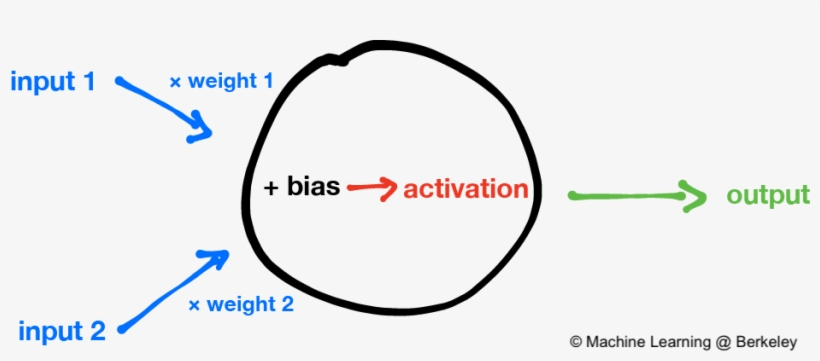
\includegraphics[width=8cm]{images/neuron.jpg}}
\end{center}
\end{frame}

\begin{frame}[fragile]{Network}
Many neurons together make up a layer of which there are three types
\begin{itemize}
	\item Input
	\item Output
	\item Hidden
\end{itemize}
During training the weights in the hidden layer will be adjusted in a process known as Back Propagation in order to improve accuracy
\begin{center}
{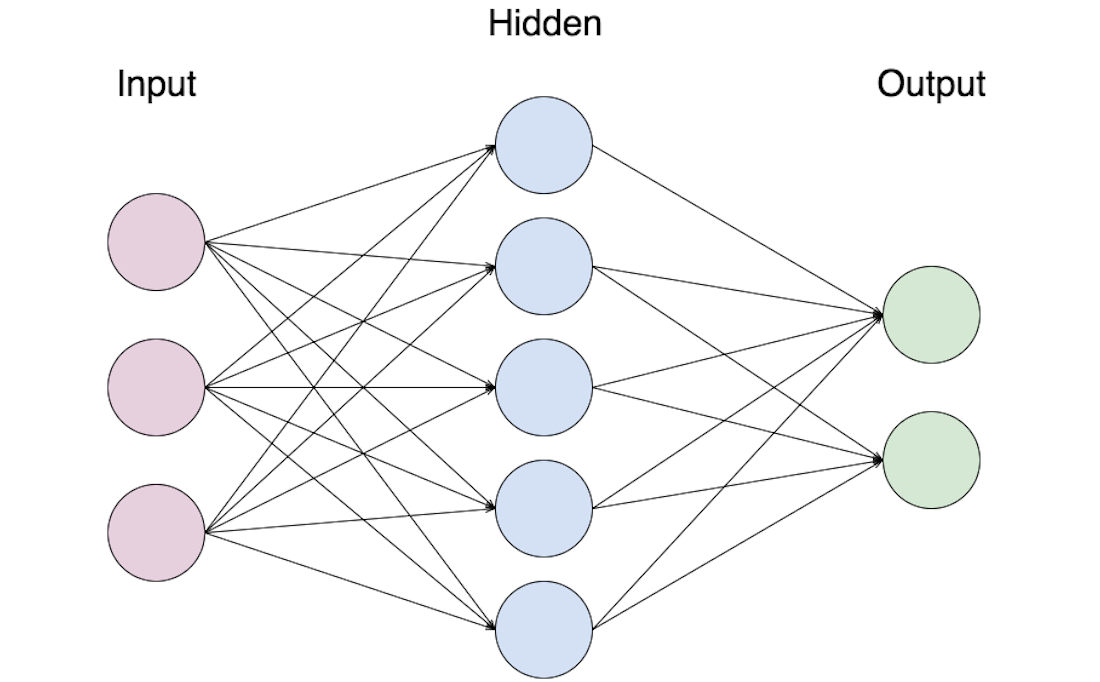
\includegraphics[width=5cm]{images/neuralnetdiagram.png}}
\end{center}
\end{frame}

\begin{frame}[fragile]{Gradient Descent}
Gradient Descent is how the Machine Learns! This is a feedback cycle that aims to minimize the loss function by descending down the derivative of the lost function until you reach the minimum
\begin{example}
	\begin{equation*}
	\left( {GD} \right):{\hat \beta ^{\left( {t + 1} \right)}} = {\hat \beta ^{\left( t \right)}} - \gamma \nabla {E_n}\left[ {\ell \left( {y,\hat y\left( {{{\hat \beta }^{\left( t \right)}}} \right)} \right)} \right]
	\end{equation*}
	\end{example}
\end{frame}

\section{Making our Model}

\begin{frame}[fragile]{NFL Play-By-Play Analysis}
Now it is time to create our Tensorflow Model! We're using play-by-play data from the NFL 2021-2022 season gathered from \href{http://nflsavant.com/about.php}{\tt \textcolor{blue}{NFLSavant}}. Let's try to create a model that predicts whether the next play is going to be a first down given data. 
\begin{center}
{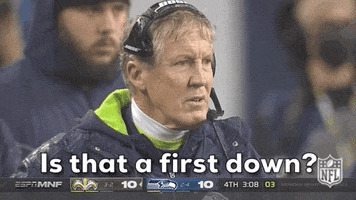
\includegraphics[width=8cm]{images/pete.jpg}}
\end{center}
\end{frame}


\section{Conclusion}

\begin{frame}{Takeaways}
For Data Engineering
\begin{itemize}
	\item Drop values in order to get rid of empty, redundant, or outlying/influential points
	\item Encode Categorical Data using techniques like one-hot encoding
	\item Normalize your data before using it.
\end{itemize}
For Building and Analyzing Model
\begin{itemize}
	\item Use sigmoid activation function for output layers with one node
	\item Use binary cross-entropy as a loss function
	\item Watch out for overfitting
\end{itemize}
\end{frame}

\begin{frame}{Shameless Promo}

Thank you very much for attending! The material for this workshop is accessible here --> \href{https://github.com/PranavTavildar1/Tensorflow-For-Sports-Analytics}{\tt \textcolor{blue}{Session Material}}.
\par
Join UConn Data Science Club! 
\par
Our UConntact --> \href{https://uconntact.uconn.edu/organization/datascience}{\tt \textcolor{blue}{Our UConntact}}.
\par
Our Discord --> \href{https://discord.gg/UJCZjXUWzg}{\tt \textcolor{blue}{Discord}}.

\end{frame}


\end{document}

